% classes
\documentclass{article}

% packages
\usepackage{graphicx}
\usepackage{fancyhdr} % Required for custom headers
\usepackage{lastpage} % Required to determine the last page for the footer
\usepackage{extramarks} % Required for headers and footers
\usepackage{courier} % Required for the courier font

\usepackage{color}
\usepackage{enumitem}

\usepackage{hyperref}

\usepackage{wrapfig}

\usepackage{fancyvrb}
\newenvironment{Schunk}{}{}
\DefineVerbatimEnvironment{Sinput}{Verbatim}{fontshape=sl}

\newcommand{\code}[1]{\texttt{#1}}
% \newcommand{\pkg}[1]{\mbox{\textbf{#1}}}
\newcommand{\pkg}[1]{\mbox{\texttt{#1}}}
\newcommand{\proglang}[1]{\textsf{#1}}

% page layout

\topmargin=-0.45in
\evensidemargin=0in
\oddsidemargin=0in

\textwidth=6.5in
\textheight=9.0in

\headsep=0.25in

\linespread{1.1} % Line spacing
 
\pagestyle{fancy}

% headers and footers

\fancyhf{}

\lhead{INTR 100 Breaking Intuition}

\rhead{
\includegraphics[width=0.045\textwidth]{wmlogo.jpg}}

\cfoot{Page \thepage}


% document body

\begin{document}

\vspace*{.01mm}

\begin{center}

\Large{\textcolor{blue}{\textbf{Lab 1.}  Why William \& Mary?}}

\vspace{4mm}

\textit{Due by noon on Friday, September 11th}\\

\end{center}

\begin{figure}[h!]
\begin{center}
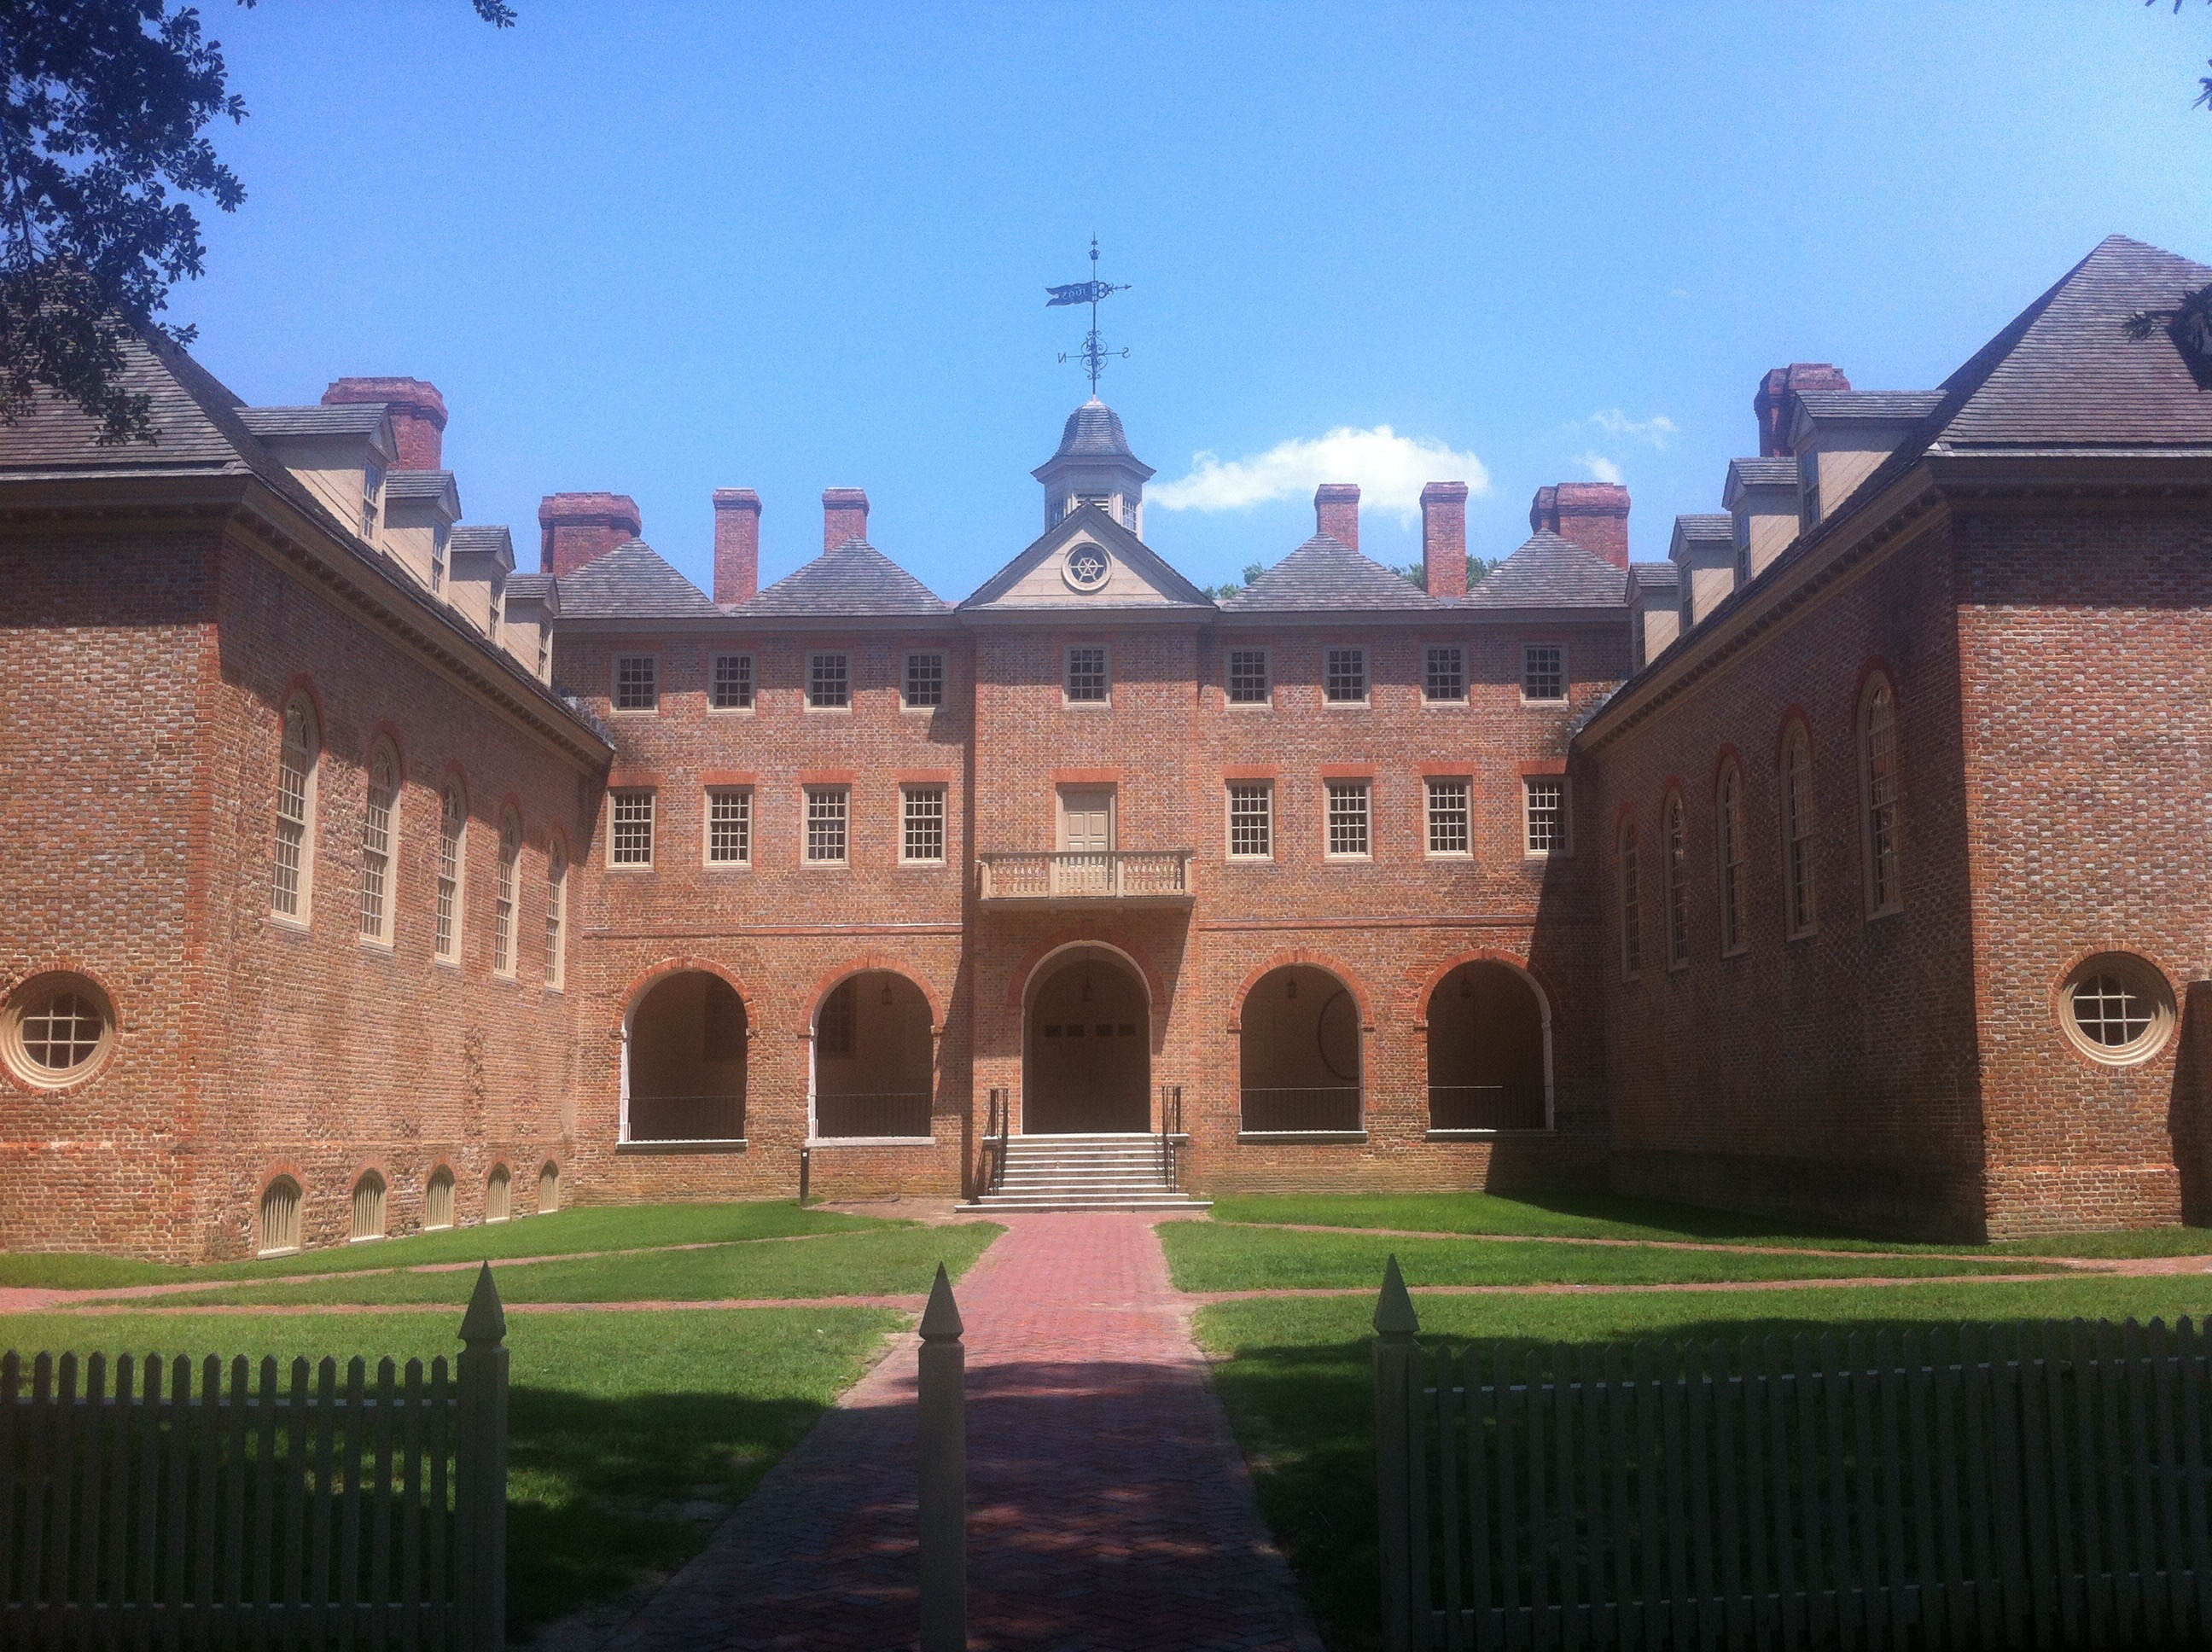
\includegraphics[width=1.0\textwidth]{wm_wrenbldg.jpg}

\end{center}
\end{figure}

\setlength{\parindent}{0cm}

\large{\textit{"I look to the diffusion of light and education as the resource most to be relied on for ameliorating the condition, promoting the virtue, and advancing the happiness of man.  %That every man shall be made virtuous, by any process whatever, is, indeed, no more to be expected, than that every tree shall be made to bear fruit, and every plant nourishment.  The brier and the bramble can never become the vine and the olive; but their asperities may be softened by culture, and their properties improved to usefulness in the order and economy of the world."}
\begin{flushright}
Letter from Thomas Jefferson to C.C. Blatchley, 1822
\end{flushright}
}

\newpage

% Enumerate the Laboratory Objectives

\large{\textbf{Laboratory in Brief:}}

\vspace{4mm}

\setlength{\leftskip}{1cm}

\setlength{\parindent}{0cm}

The purpose of this laboratory is to think about ways to justify a decision using data that is openly accessible via a web browser.  We will continue your introduction to the statistical programming language \proglang{R} and some of its basic methods.  You may be asking yourself, "Will I really need to defend my choice to attend William \& Mary for another two weeks?"  The goal of this assignment is not only to encourage you to consider the College you have chosen, but also to begin thinking about how to obtain, import, manage and use data in support of your (very good) decision.

\vspace{4mm}

\setlength{\leftskip}{0cm}

\large{\textbf{Goals of this Laboratory:}}

\begin{enumerate}[leftmargin=15mm]

\item To retrieve data from an open access server via a web browser and create a \code{.csv} (comma-separated values) file for saving to your William \& Mary \code{H:\textbackslash\textbackslash} drive.

\item To begin understanding how to think about and describe data, while also continuing our introduction to the statistical programming language \proglang{R}.

\item To create plots for incorporation into a visualization that supports a decision using a given data set.

\end{enumerate}

\large{\textbf{Session 1: Monday, August 31st}}

\vspace{4mm}
\setlength{\leftskip}{1cm}
\textit{Step-by-step instructions: first, lets acquire the data by using our web browser}

\begin{enumerate}[leftmargin=15mm]

\item With your browser go to the National Center for Education Statistics' Data Center website.  You should be able to simply click on the following link.\\ 
\url{https://nces.ed.gov/ipeds/datacenter/}

\item On the left side of the webpage find the \textbf{Download Custom Data Files} link and select it.  
\begin{flushright}{
\includegraphics[width=0.61\textwidth]{homepage.png}}\end{flushright}
 
\item After selecting the \textbf{Download Custom Data Files} link you will be asked \textit{What data would you like to access?"} Under the \textit{Provisional Release Data} and below the \textit{For additional years of data:} go ahead and select \textbf{Use final release data} and then select 
\includegraphics[width=0.125\textwidth]{continue.png}.

\item Next you will you will be asked \textit{"How would you like to select institutions to include in your data file/report?"}  Of the three options available, place your cursor over the link for \textbf{By Groups}, so that a sub-window appears, then choose \textbf{EZ Group}.

\item After selecting \textbf{EZ Group} you will be presented with options under the heading \textit{Data Collection: 2013}.  The first line will present you with four options, choose \textbf{U.S. only}.  Once you select \textbf{U.S. only}, the grey bar to the right should automatically update to indicate that \textit{7597} institutions will be selected.  Then go ahead and choose 
\includegraphics[width=0.1\textwidth]{search.png}.

\item Now your institutions have been selected and you should have a list of the first 20 of the 7597 U.S. higher education institutions that you will be selecting.  On this page, you only need to select the 
\includegraphics[width=0.125\textwidth]{continue.png} button that is found following the statement \textit{When you have finished selecting institutions} 
\includegraphics[width=0.125\textwidth]{continue.png} \textit{to Step 2 - Select Variables}.

\item On the next page you will select the variables that will be downloaded to your local machine as a \code{.csv} file.  Scroll down past \textit{Available Years} and find the 
\includegraphics[width=0.04\textwidth]{plus.png} to the left of \textbf{Frequently used/Derived variables} and click on it so all the sub options appear.  Then expand the 
\includegraphics[width=0.04\textwidth]{plus.png} to the left of \textbf{Institutions}.  This same field appears again (\textit{seems like it might be a website typo}) so you will need to expand it a second time.  Then once you have fully expanded the field, choose \textbf{State abbreviation}. \begin{flushright}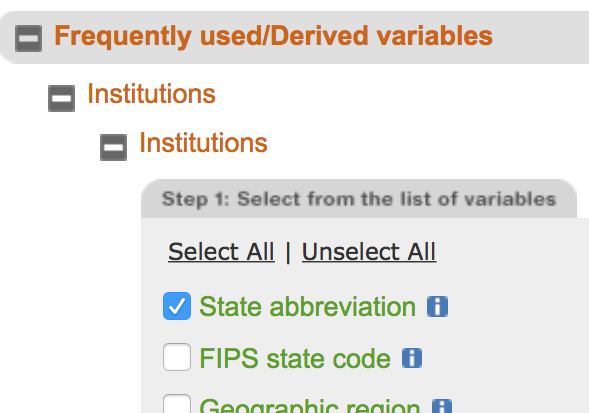
\includegraphics[width=0.35\textwidth]{state.png} \end{flushright}

\item Once you have selected the \textbf{State abbreviation} box go back to the top level \textbf{Frequently used/Derived variables} and select the 
\includegraphics[width=0.04\textwidth]{plus.png} to the left of the \textbf{Total cost of attendance} field.  This field should expand and present you with several check box options under the title \textit{Price}.  Select the first four fields named \textbf{Tuition and fees}, each one for a different year: \textbf{2010-11, 2011-12, 2012-13, 2013-14}. \begin{flushright} 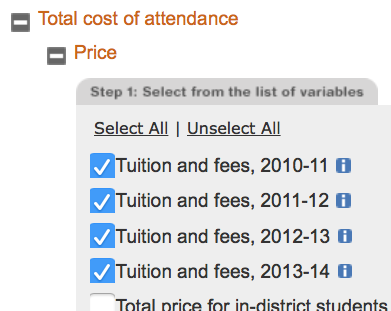
\includegraphics[width=0.35\textwidth]{cost.png} \end{flushright}

\item Now you will want to go back to the top level again \textbf{Frequently used/Derived variables} and this time expand the 
\includegraphics[width=0.04\textwidth]{plus.png} next to \textbf{Revenues and expenditures: Fiscal year 2013}.  Then under that heading expand \textbf{Expenses for salaries, wages and nbenefits as a percent of total expenses, by function} where you will need to choose the first four options \textbf{Salaries, wages and benefit expenses for core expenses, instruction, research and public service} \begin{flushright}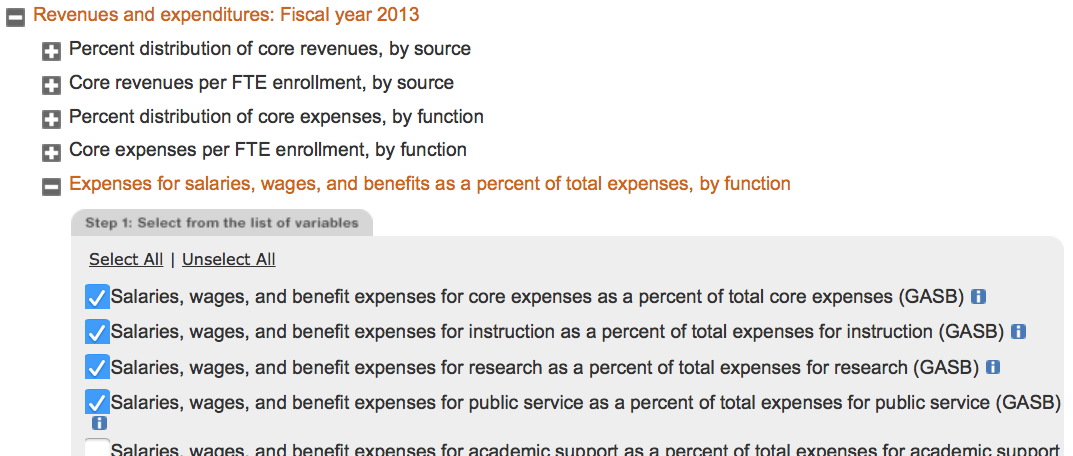
\includegraphics[width=0.7\textwidth]{core.png} \end{flushright}

\item Finally, scroll back up to the top of the page and click 
\includegraphics[width=0.125\textwidth]{continue2.png}.

\item On this final page, the IPEDS Data Center web page will ask in what format do you want your data.  In the box labeled \textit{Year 2013}, and under the heading \textit{Download as single file for:}, off to the right select the \textbf{CSV button}.\begin{flushright}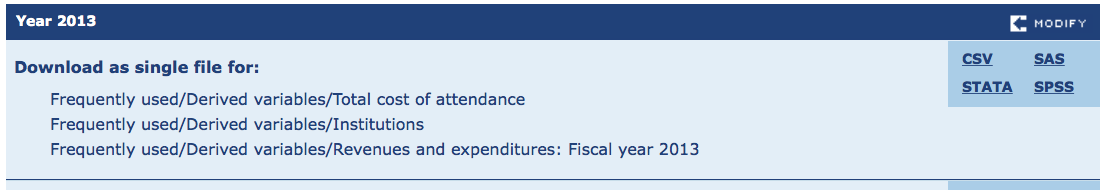
\includegraphics[width=0.75\textwidth]{csv.png}\end{flushright}

\item Selecting the \textbf{CSV button} will download a folder that is named \texttt{CSV\_} followed by a series of numbers to your download folder.  Go ahead and move that folder to your desktop and open it up.  Inside this folder you will find a \code{.csv} file and \code{.html} file.  Go ahead and move the \code{.csv} file to your William \& Mary \code{H:\textbackslash\textbackslash} drive, then rename it to \texttt{lab1\_data.csv} or something similar.

\item Then we can open your \code{.csv} file in Microsoft Excel and have a brief look.

\item Finally, let's import your \code{.csv} file into \proglang{R} and create an object.

\begin{enumerate}[label=\Alph*.  ]

\item In your William \& Mary \code{H:\textbackslash\textbackslash} drive, create a New Folder and name it \code{lab1} or something similar.

\item Open \proglang{R} or R Studio

\item Create a new script file.  Go to the \textbf{File} menu and choose \textbf{New Document}.  Then save this \code{.R} script file to your William \& Mary \code{H:\textbackslash\textbackslash}\code{lab1} folder, and name it \texttt{lab1\_script.R} or something similar.

\item One of the first lines of code in your script file should tell \proglang{R} where your working directory is located, which in this case is \code{H:\textbackslash\textbackslash}\code{lab1}.  The working directory is the default location where \proglang{R} will look for a file that has been identified as part of a command.  While we could specify the full path of our file location, once we set the working directory, \proglang{R} will automatically know where to find our \code{.csv} file.

\begin{Schunk}
\begin{Sinput}

R> setwd("H:\\lab1")

\end{Sinput}
\end{Schunk}

\item After setting your working directory, now we should be able to import our \code{.csv} file into R by using the \code{read()} command in \proglang{R} and typing the following.

\begin{Schunk}
\begin{Sinput}

R> data <- read.csv("lab1.csv")

\end{Sinput}
\end{Schunk}

Now we have created an object named \code{data}.  By keeping our source data external to \proglang{R} and then importing it and creating a new object, we have greatly enhanced the reproducibility of our work and advancing one of the fundamental principals of the scientific method.  From this point forward our work is in our code, while the data remains in its original state and does not change. \\ %While today, we are using a web browser and graphical user interface to retrieve the data, often, this step is also part of your code.  In this case, the first step is not necessarily to import the data, but to access and retrieve it using an \textit{application program interface} (API) from a server.

\item Finally we can think about the structure of the \proglang{R} object we have created.  The \code{str()} command is used to determine the type of object, and several other characteristics about that object.  Rather than saving the \code{str()} command in our code, we can simply type it directly into the console.

\begin{Schunk}
\begin{Sinput}

R> str(data)

\end{Sinput}
\end{Schunk}

\proglang{R} informs us that our object is a \code{data.frame} with \code{7597 obs.} of \code{12 variables}.  Then \proglang{R} lists the name of each variable in our \code{data.frame}, tells us the variable name, the data type for that variable and then prints the first few observations found in that variable.

\end{enumerate}

\end{enumerate}

% Step by Step Instructions for Day 2

\setlength{\leftskip}{0cm}

\large{\textbf{Session 2: Wednesday, September 2nd}}

\vspace{4mm}
\setlength{\leftskip}{1cm}
\textit{Step-by-step instructions: now let's modify \& describe our data}

\begin{enumerate}[leftmargin=15mm]

\item For starting out on day 2, lets think about the \proglang{R} object we have created a bit more.  We can type in \code{str(data)} as we did at the end of Session 1, or we could also use the \code{names()} command, and \proglang{R} will give us the names of each of the 12 variables.

\begin{Schunk}
\begin{Sinput}

R> names(data)

\end{Sinput}
\end{Schunk}

Many of these names are long and confusing, so it would be helpful to rename our variables and make them more manageable.  To do this, we will create a new \proglang{R} object that contains each of the new names that will be used to replace the 12 existing ones.  When doing this, it is important that the new names are listed in the same order as the existing ones as contained in the \code{data.frame}.

\begin{Schunk}
\begin{Sinput}

R> data_names <- c("id", "name", "year", "tuition10_11", 
"tuition11_12", "tuition12_13", "tuition13_14", "state", 
"core_exp", "instructional_exp", "research_exp", 
"publicservice_exp")

\end{Sinput}
\end{Schunk}

We can then type \code{data\_names} directly into the console and \proglang{R} will return the same names we just typed when creating that object.

\item Again we use the \code{names()} function to replace the existing names with the new ones.

\begin{Schunk}
\begin{Sinput}

names(data) <- data_names

\end{Sinput}
\end{Schunk}

Now we can type \code{str(data)} to verify that our variables have been renamed.

\item Next we will use \proglang{R} to examine our data.  First, let's think about how our data set can be described spatially.  To do this we can consider the state where each institution is located by identifying the appropriate variable that provides this information.  Using the \code{str(data)} command again should begin to facilitate our inquiry.

\begin{Schunk}
\begin{Sinput}

> str(data)
'data.frame':	7597 obs. of  12 variables:
 $ id               : int  100654 100663 100690 100706 100724 100733 100751 100760 100812 100830 ...
 $ name             : Factor w/ 7457 levels "A & W Healthcare Educators",..: 100 6639 240 6640 103 6641 6388 1101 405 423 ...
 $ year             : int  2013 2013 2013 2013 2013 2013 2013 2013 2013 2013 ...
 $ tuition10_11     : int  5800 5806 8360 7492 7164 NA 7900 2700 NA 6620 ...
 $ tuition11_12     : int  6828 6264 8720 8094 8082 NA 8600 2700 NA 7580 ...
 $ tuition12_13     : int  7182 6798 6800 8794 7932 NA 9200 4140 NA 8150 ...
 $ tuition13_14     : int  7182 7206 6870 9192 8720 NA 9450 4200 NA 8750 ...
 $ state            : Factor w/ 51 levels "Alabama","Alaska",..: 1 1 1 1 1 1 1 1 1 1 ...
 $ core_exp         : int  48 68 NA 68 44 99 67 43 61 59 ...
 $ instructional_exp: int  78 83 NA 80 73 NA 77 83 77 92 ...
 $ research_exp     : int  52 60 NA 69 33 NA 52 NA NA 56 ...
 $ publicservice_exp: int  60 54 NA 45 14 NA 70 17 NA 49 ...
 
\end{Sinput}
\end{Schunk}

We can see this \code{data.frame} object has 12 variables, the name for each one listed (as we had previously renamed them), following a \code{\$} sign.  The variable \code{\$state} appears to be the correct one to determine the location for each of the \code{7597 obs.}  In order to return a table that aggregates all institutions according to state, we use the \code{table()} command by executing the following code.

\begin{Schunk}
\begin{Sinput}

R> table(data$state)

\end{Sinput}
\end{Schunk}

Now we have introduced an additional wrinkle to our  code.  Instead of simply executing a function that addresses only an object, we have also qualified that object by using the \code{\$} sign.  The \code{\$} sign is used to indicate which of the variables within the object is being used as part of the executed function.  In this case when we use \code{table(data\$state)} \proglang{R} totals the number of institution located in each state.

\begin{Schunk}
\begin{Sinput}
             Alabama               Alaska              Arizona             Arkansas           California 
                  93                   12                  146                   88                  789 
            Colorado          Connecticut             Delaware District of Columbia              Florida 
                 140                  100                   21                   25                  402 
             Georgia               Hawaii                Idaho             Illinois              Indiana 
                 199                   28                   44                  320                  139 
                Iowa               Kansas             Kentucky            Louisiana                Maine 
                  96                   96                  117                  128                   43 
            Maryland        Massachusetts             Michigan            Minnesota          Mississippi 
                 105                  197                  204                  149                   64 
            Missouri              Montana             Nebraska               Nevada        New Hampshire 
                 226                   31                   53                   53                   44 
          New Jersey           New Mexico             New York       North Carolina         North Dakota 
                 173                   52                  481                  199                   30 
                Ohio             Oklahoma               Oregon         Pennsylvania         Rhode Island 
                 383                  149                   99                  405                   24 
      South Carolina         South Dakota            Tennessee                Texas                 Utah 
                 113                   31                  189                  478                   88 
             Vermont             Virginia           Washington        West Virginia            Wisconsin 
                  28                  178                  127                   79                  127 
             Wyoming 
                  12
\end{Sinput}
\end{Schunk}

\item We can also ask \proglang{R} to give us the summary statistics of all observations for a single variable.  To do this, we use the \code{summary()} command and again identify that variable by using the \code{\$} operator.

\begin{Schunk}
\begin{Sinput}

R> summary(data$tuit13_14)

   Min. 1st Qu.  Median    Mean 3rd Qu.    Max.    NA's 
     80    5242   12110   14140   18050   64900    3424 

\end{Sinput}
\end{Schunk}

In this case, \proglang{R} has returned basic descriptive statistics, including the mean, median, 1st and 3rd quartiles, as well as the minimum and the maximum for the variable total tuition and costs for the school year 2013 to 2014.  The last column \code{NA's} is a special designation in \proglang{R} that counts the total number of observations within a variable that do not have an outcome.  It literally stands for \textit{Not Available}.  Keep in mind that an observation outcome \code{NA} is different from a 0 or an indication such as None.

\item We can also do the same thing, but instead of calculating the summary statistics for all U.S. educational institutions, we can subset only those schools that are located in the state of Virginia.  The simplest way to do this is by using the \code{subset()} command.

\begin{Schunk}
\begin{Sinput}

R> subset(data, state == "Virginia")
     
\end{Sinput}
\end{Schunk}

Notice the \code{subset()} command introduces another, new wrinkle to our code.  Rather than using the \code{\$} operator as before, this time, first we indicate the object, then a second qualifying statement designates the variable, in this case \code{state == "Virginia"}. \\

Additionally, it would be helpful to have the summary statistics for our subset of the data.  First, we create a new object using the assignment operator and then execute our \code{summary()} command once again for our subset of the data we have just created.

\begin{Schunk}
\begin{Sinput}

R> va_data <- subset(data, state == "Virginia")
R> summary(va_data$tuit13_14)

Min. 1st Qu.  Median    Mean 3rd Qu.    Max.    NA's 
   3169    7922   14670   14920   18050   45320      60

\end{Sinput}
\end{Schunk}

Now we can compare the various summary statistics for all the institutions in Virginia with those for the entire United States of America.  How does tuition in Virginia compare with the rest of the country?

\item We can also isolate those institutions in Virginia that are above the national mean?  We do this by first creating an object that represents the national average of total tuition and costs for the year 2013 to 2014.  Notice the qualifying statement \code{na.rm = TRUE}, which stands for NA's remove.  This statement removes all of the observations that have unavailable outcomes and permits \proglang{R} to return the correct mean for the chosen variable. 

\begin{Schunk}
\begin{Sinput}

R> us_mean <- mean(data$tuition13_14, na.rm = TRUE)
R> va_above_avg <- subset(va_data, tuition13_14 > us_mean)

\end{Sinput}
\end{Schunk}

\item To see if William \& Mary is above the national average, just type the object name  \code{va\_above\_avg} and look through the output or you can also type

\begin{Schunk}
\begin{Sinput}

R> subset(data, name == "College of William and Mary")

\end{Sinput}
\end{Schunk}

\item We can also use the \code{subset()} command to find the least expensive school in the country, while using the \code{class()} command will inform us of the object type.  In this case, our institution name is returned as a factor, when all we need is the school's name.  We can use \code{as.character()} to convert the name of the school from factor to character.

\begin{Schunk}
\begin{Sinput}

R> min(data$tuition13_14, na.rm = TRUE)
R> min_cost <- min(data$tuition13_14, na.rm = TRUE)
R> min_obs <- subset(data, tuition13_14 == min_cost)
R> min_obs$name
R> class(min_obs$name)
R> min_name <- as.character(min_obs$name)
R> min_name
R> class(min_name)

\end{Sinput}
\end{Schunk}

Sometimes \code{subset()} functions requirement of using a logical argument can be a nuisance.  A more advanced approach to solving the same problem is to extract observations using brackets.  The \code{[} and \code{]} brackets are also called subscripting operators.

\begin{Schunk}
\begin{Sinput}

R> data[which.max(data$tuition13_14),]
R> data[which.max(data$tuition13_14),]$name
R> as.character(data[which.max(data$tuition13_14),]$name)

\end{Sinput}
\end{Schunk}

As we can see, we accomplished the same result with only two lines of code using the \code{[} and \code{]} brackets instead of the \code{subset()} command.  Subscripting is one of the most powerful tools available in \proglang{R} due to its speed and widespread applicability.  Type \code{?Subscript} or \code{?Extract} to read the help page on how to use the \code{[} and \code{]} brackets as operators.

%We need to e-mail a short instructional paper on using brackets for the students to read in preparation for Day 3

\end{enumerate}

% Step by Step Instructions for Day 3

\setlength{\leftskip}{0cm}

\large{\textbf{Session 3: Monday, September 7th}}

\vspace{4mm}
\setlength{\leftskip}{1cm}
\textit{Step by Step Instructions: now let's analyze \& plot our results}

\begin{enumerate}[leftmargin=15mm]

\item Now, we're going to do some basic analysis that you can include on your revised infographic.  Note the goal of this \proglang{R} tutorial is not to create beautiful visualisations though \proglang{R} can do that.  Rather, we want to extract data you can then use in visme to improve your original infographic.  Let's do something very simple to start: how does the percentage increase of William and Mary's tuition compare to (a) all schools, and (b) Virginia schools from 2010 to the 2013-2014 school year?

\item First, let's calculate this for William \& Mary.

\begin{Schunk}
\begin{Sinput}

R> wm_tuition1314 <- data[which(data$name == "College of 
William and Mary"), ]$tuition13_14
R> wm_tuition1213 <- data[which(data$name == "College of 
William and Mary"), ]$tuition12_13
R> wm_tuition1112 <- data[which(data$name == "College of 
William and Mary"), ]$tuition11_12
R> wm_tuition1011 <- data[which(data$name == "College of 
William and Mary"), ]$tuition10_11

R> wm_change14 <- wm_tuition1314 / wm_tuition1213
R> wm_change13 <- wm_tuition1213 / wm_tuition1112
R> wm_change12 <- wm_tuition1112 / wm_tuition1011

R> wm_change <- mean(c(wm_change14, wm_change13, wm_change12))

R> wm_change
[1] 1.083435

\end{Sinput}
\end{Schunk}

This gives us the \textit{average annual change} in tuition costs for the time period from the school year 2010 and 2011 until the school year 2013 and 2014.  Note there are only three annual intervals to average since we have not included the tuition costs for the years before 2010 or after 2014.  The \code{c()} operator is another new command that literally means to combine.  Here we use the \code{c()} to find the mean of the three combined objects.

\item Now, let's calculate the average change for every other school.  This is the first time we will add a new column to our data frame.  We can review our existing variable names, as we did at the beginning of this laboratory by again using the \code{str()} or \code{names()} command.

\begin{Schunk}
\begin{Sinput}

R> str(data)

\end{Sinput}
\end{Schunk}

\item Now, let's create a new variable that describes the \textit{average annual change} in tuition costs for all institutions during the same period of time (as we have just done for William \& Mary).

\begin{Schunk}
\begin{Sinput}

R> data$us_change14 <- data$tuition13_14 / data$tuition12_13
R> data$us_change13 <- data$tuition12_13 / data$tuition11_12
R> data$us_change12 <- data$tuition11_12 / data$tuition10_11

R> data$us_change <- (data$us_change14 + data$us_change13 + 
data$us_change12) / 3

R> data$us_change

R> mean(data$us_change, na.rm = TRUE)
[1] 1.046987

\end{Sinput}
\end{Schunk}

\item Note, there are several new names in our data.frame when we type \code{names(data)}.  Let's summarize the annual change variable now:

\begin{Schunk}
\begin{Sinput}

R> summary(data$us_change)
   Min. 1st Qu.  Median    Mean 3rd Qu.    Max.    NA's 
  0.709   1.023   1.039   1.047   1.057   8.701    3592 

\end{Sinput}
\end{Schunk}

\item Let's do a comparison between the tuition in 2014 and the percent of that money spent on instructors salaries.  First, let's look it up for William \& Mary:

\begin{Schunk}
\begin{Sinput}

R> wm <- subset(data, name == "College of William and Mary")
R> wm$instructional_exp

\end{Sinput}
\end{Schunk}

\item And second, let's compare that to the national average:

\begin{Schunk}
\begin{Sinput}

R> summary(data$instructional_exp)

\end{Sinput}
\end{Schunk}

\item Finally, let's plot out all schools tuition in 2014 contrasted to the \% of tuition they spend on instructors salary.

\begin{Schunk}
\begin{Sinput}

R> plot(data$instructional_exp, data$tuition13_14)

\end{Sinput}
\end{Schunk}

\item That on it's own isn't particularly helpful, as it's hard to see patterns with outliers and without knowing which dot is William \& Mary.  It's also probably more fair to compare to only Virginia schools, so let's drop out everything that isn't Virginia and label W\&M in an appropriate color.  First, re-use the old VAcolleges dataset you made:

\begin{Schunk}
\begin{Sinput}

R> plot(va_data$instructional_exp, va_data$tuition13_14)

\end{Sinput}
\end{Schunk}

\item Now, let's label just W\&M save this figure (click the export button above the chart) as you will be turning it in!

\begin{Schunk}
\begin{Sinput}

R> wm_plot <- data[which(data$name=="College of William and 
Mary"),]
R> points(wm_plot$instructional_exp, wm_plot$tuition13_14, 
col="green")

\end{Sinput}
\end{Schunk}

\end{enumerate}

% Step by Step Instructions for Day 4

\setlength{\leftskip}{0cm}
 
\large{\textbf{Session 4: Wednesday, September 9th}}

\vspace{4mm}
\setlength{\leftskip}{1cm}
\textit{Step by Step Instructions: Lab Questions}

\begin{enumerate}[leftmargin=15mm]

\item Calculate which two states have the most colleges, and how many does each one have?

\item Calculate the mean tuition cost for the US and for Virginia?  Does Virginia have a higher or lower average tuition cost than the rest of the USA?  What is this difference?

\item Calculate the 2010-2011, 2011-2012, 2012-2013, and 2013-2014 Tuition and Annual Percent Change for William \& Mary, all Universities in Virginia, and all Universities in the USA.

\item Create a graph showing USD invested in instruction as compared with tuition costs and highlight William \& Mary.  Create a similar chart considering the mean of these two values for all Universities in Virginia and all Universities in the USA.

\item Calculate what are the most and least expensive Universities in Virginia and the USA. 

\item Attach a printed copy of your "visme" visualisation to this document, or submit it electronically.  What variable did you include that was not explicitly a part of this lab?  What challenges did you have in retrieving it, and how did you use it to illustrate William and Mary is an exceptional (or, crazy!) choice of where to get your degree?

\end{enumerate}

\vspace{4mm}
\setlength{\leftskip}{0cm}
\textit{Stretch Goals}

Made it this far?  Want to try to go even farther?  Just want to learn?  Try any of the following to really impress us, it won't count for your grade, but it'll give you a leg up on future assignments:
\begin{itemize}
\item In your download, ask for the "latitude" and "longitude" columns, then plot colleges following this tutorial: \url{http://www.milanor.net/blog/?p=594}
\item Examine how US schools compare to international schools.
\item Make similar comparisons with a different dataset ? i.e., try
\end{itemize}


% Final Output from Laboratory

\setlength{\leftskip}{0cm}

\large{\textbf{Final Output for Submission}}

\vspace{4mm}
\setlength{\leftskip}{1cm}
\textit{Due by noon on Friday, November 13th:}
\vspace{2mm}

...  Make certain the Final Report meets the following criteria.

\begin{itemize}

\item One visme visualization including output from Session 2 and Session 3 as well as answers to the questions from Session 4

\end{itemize}

% Grading

\setlength{\leftskip}{0cm}

\textbf{Grading}

\vspace{4mm}

\setlength{\leftskip}{1cm}

\setlength{\parindent}{0cm}

This lab will be graded based on your visme visualization.
%----------------------------------------------------------------------------------------

\end{document}